
\documentclass[12pt]{article}
%%%%%%%%%%%%%%%%%%%%%%%%%%%%%%%%%%%%%%%%%%%%%%%%%%%%%%%%%%%%%%%%%%%%%%%%%%%%%%%%%%%%%%%%%%%%%%%%%%%%%%%%%%%%%%%%%%%%%%%%%%%%%%%%%%%%%%%%%%%%%%%%%%%%%%%%%%%%%%%%%%%%%%%%%%%%%%%%%%%%%%%%%%%%%%%%%%%%%%%%%%%%%%%%%%%%%%%%%%%%%%%%%%%%%%%%%%%%%%%%%%%%%%%%%%%%
\usepackage{amsmath,amsthm}
\usepackage[latin1]{inputenc}
\usepackage[T1]{fontenc}
%\usepackage{minionpro}
\usepackage{array,graphicx}

\setcounter{MaxMatrixCols}{10}
%TCIDATA{TCIstyle=LaTeX article (bright).cst}

%TCIDATA{OutputFilter=LATEX.DLL}
%TCIDATA{Version=5.00.0.2570}
%TCIDATA{<META NAME="SaveForMode" CONTENT="1">}
%TCIDATA{Created=Monday, January 29, 2007 11:45:31}
%TCIDATA{LastRevised=Friday, November 30, 2007 08:35:24}
%TCIDATA{<META NAME="GraphicsSave" CONTENT="32">}
%TCIDATA{<META NAME="DocumentShell" CONTENT="Exams and Syllabi\SW\Assignment">}
%TCIDATA{Language=American English}

\setlength{\topmargin}{-0.3in} \setlength{\textheight}{8.75in}
\setlength{\oddsidemargin}{0.0in} \setlength{\evensidemargin}{0.0in}
\setlength{\textwidth}{6.5in}
\def\labelenumi{\arabic{enumi}.}
\def\theenumi{\arabic{enumi}}
\def\labelenumii{(\alph{enumii})}
\def\theenumii{\alph{enumii}}
\def\p@enumii{\theenumi.}
\def\labelenumiii{\arabic{enumiii}.}
\def\theenumiii{\arabic{enumiii}}
\def\p@enumiii{(\theenumi)(\theenumii)}
\def\labelenumiv{\arabic{enumiv}.}
\def\theenumiv{\arabic{enumiv}}
\def\p@enumiv{\p@enumiii.\theenumiii}
\pagestyle{plain}
\pagestyle{plain} \setcounter{secnumdepth}{3}
\newcommand{\D}{\mathop{\mathrm{d\mathstrut}}\nolimits\!}
\newcommand{\dt}{\D t}
\newcommand{\dz}{\D z}
\newcommand{\E}{\mathop{\mathrm{E\mathstrut}}\nolimits}
\newcommand{\Var}{\mathop{\mathrm{Var\mathstrut}}\nolimits}
\newcommand{\sd}{\mathop{\mathrm{sd\mathstrut}}\nolimits}
\newcommand{\diag}{\mathop{\mathrm{diag\mathstrut}}\nolimits}
\newcommand{\Cov}{\mathop{\mathrm{Cov\mathstrut}}\nolimits}
\newcommand{\Corr}{\mathop{\mathrm{Corr\mathstrut}}\nolimits}
\newtheorem{definition}{Definition}
\newtheorem{proposition}{Proposition}
\newtheorem{conjecture}{Conjecture}
\newtheorem{moment}{Empirical regularity}
\newtheorem{insight}{Qualitative prediction}



\begin{document}

\title{A Spatial Explanation for the Balassa--Samuelson Effect\thanks{\textsc{Preliminary and incomplete. Please do not circulate.}}}
\author{P\'eter Kar\'adi\thanks{New York University. E-mail: peter.karadi@nyu.edu}~ and Mikl\'os Koren\thanks{Princeton University. E-mail: mkoren@princeton.edu.}}
\maketitle

\begin{abstract}
We propose a model of urbanization and development to explain why the price level is higher in rich countries. There are two sectors: manufacturing, which is freely tradable, and non-tradable services, which have to locate near customers in big cities. As countries develop, total factor productivity increases simultaneously in both sectors. However, because services compete with the urban population for scarce land, labor productivity will grow slower in services than in manufacturing. Services become more expensive, and the aggregate price level becomes higher. The model hence provides a theoretical foundation for the Balassa--Samuelson assumption that productivity growth is slower in the non-tradable sector than in the tradable sector. The key implications of the model are borne out in the data: while the positive correlation between income and the price level is very strong among countries where land is scarce (densely populated, highly urban countries), there is virtually no such correlation among rural countries.
\end{abstract}

\section{Introduction}
Rich countries are more expensive than poor ones. Figure \ref{fig:penn_joint} shows
the strong correlation between aggregate price level and (PPP-adjusted) GDP per capita for 188 Penn-World-Table countries in 2000. Balassa (1964) and Samuelson
(1964) suggested a simple and powerful explanation based on the
observation that productivity growth of tradables, such as manufacturing,
tends to be faster than productivity growth of non-tradables, such as
services. Assuming that labor is perfectly mobile across sectors,
firms need to pay the same wage in both sectors in equilibrium, and
these wages are pinned down by the international price of the
tradable good and the productivity in the tradable sector.
Relatively lower non-tradable sector productivity, thereby, will
imply higher non-tradable prices. Empirical observations support the
major propositions of the model about the importance of the
non-tradable sector as well as the development of the relative
productivities and their effects on the relative prices (see e.g.
Obstfeld-Rogoff, 1996)\footnote{Hsieh and Klenow (1997) recently
argued that low PPP investment rates in poor countries come from
their low relative productivity in producing investment and tradable
goods relative to non-tradable consumption services.} Though
empirical results are also consistent with the assumption that total factor
productivity growth does tend to favor the tradable sector, the
theory falls short of providing an explanation for it.

Rich cities are more expensive than poor ones. According to \texttt{bestplaces.net}, the overall cost of living is 54 percent higher in Boston, MA than in Milwaukee, WI. The two cities are of similar size (close to 600,000 people), but the per capita income in Boston (\$28,000) is about 56 percent higher than that in Milwaukee (\$18,000). Similarly to the price differences across countries, the biggest price differences are in nontradable sectors. Healthcare is 33 percent more expensive in Boston, whereas housing is about 200 percent more expensive.\footnote{All data retrieved from \texttt{http://bestplaces.net} on January 30, 2008.} While the Balassa--Samuelson explanation has the potential to explain price differences across cities, some simple demand considerations also jump to mind. Demand for services is higher in high-income cities, while supply is limited, which drives up service prices. A scarce factor in cities that may limit the supply of services is land.\footnote{Tang (2007) offers an income-based explanation for the positive correlation between price level and GDP per capita. He does not focus on cities and the spatial distribution of economic activity, however.}

We propose a model of development and urbanization that reconciles these two facts and connects these two types of explanations. There are two sectors: manufacturing, which is freely tradable, and non-tradable services, which have to locate near customers in big cities. As countries develop, total factor productivity increases simultaneously in both sectors. However, because services compete with the urban population for scarce land, labor productivity will grow slower in services than in manufacturing. Services become more expensive, and the aggregate price level becomes higher with development.

Our model rests on three key observations.

First, land is scarcer than one might first think. The overall population density of the earth is rather low, 43 people per square kilometer.  However, population is very clustered, so the average person lives in an area with a population density of 5,700 people per square kilometer.\footnote{We used high-resolution population density data from LandScan to calculate, for the average person on earth, the number of people living within the same 30 arc second by 30 arc second area. (This is basically a population-weighted population density.) } A related observation is that in 2005, around 50 percent of the world population lived in cities.\footnote{World Development Indicators.} This suggests that the scarcity of land, which has the potential to explain price differences across cities, can also be partly responsible for price differences across countries.

Second, whether a good is tradable or not has implications not only for cross-country trade but also for within-country trade, and hence the location of production within the country. Arguably, there are many technological differences between tradable sectors such as manufacturing, and non-tradable sectors such as services. The fundamental difference, however, is that non-tradable goods or services have to be produced at the location of their consumption, whereas tradable goods and services can be produced far away from consumers, where land prices may be cheaper. Figure \ref{fig:ntcounties} shows a map of U.S.~counties, displaying the \emph{share} of employment in non-tradable sectors. Darker colors represent a higher share in non-tradable sectors. We see that non-tradable sectors locate closer to population centers than tradable sectors.\footnote{This is confirmed more formally in Section \ref{empirics}.} The implication of this observation is that non-tradable prices are more sensitive to the price of land than tradable prices.

\begin{figure}[h!]
%  \vspace*{-7em}
\centering
  % Requires \usepackage{graphicx}
  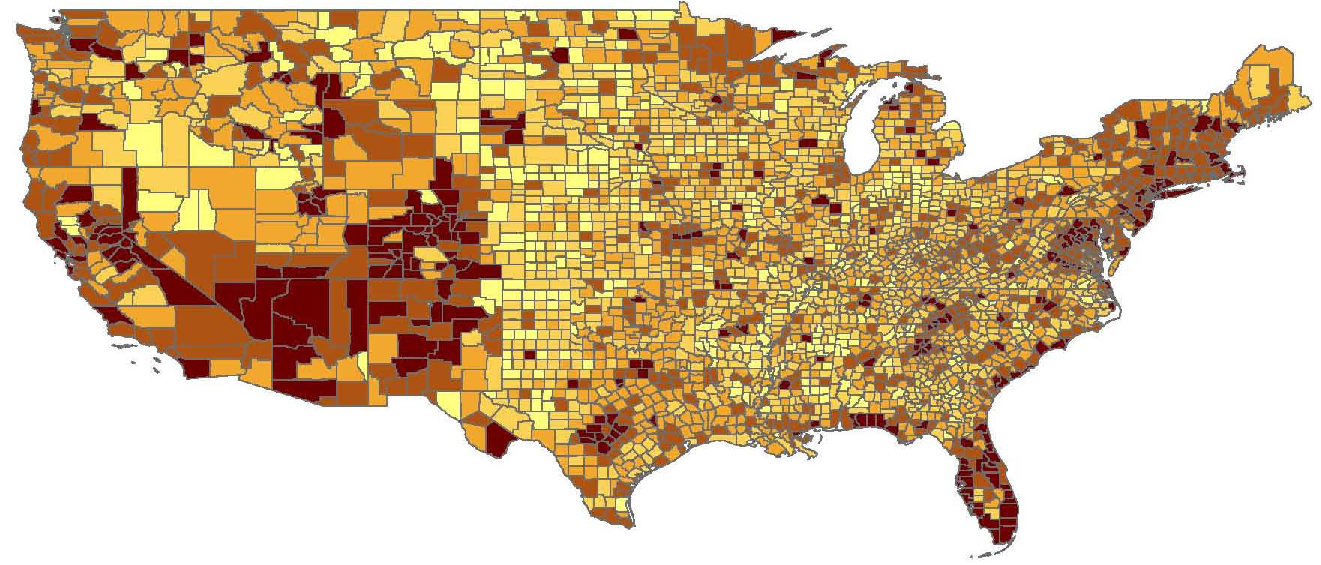
\includegraphics[width=0.7\linewidth]{figures/ntcounties}
  \vspace*{-1em}
  \caption{The share of non-traded employment in U.S.~counties}\label{fig:ntcounties}
  {\small\emph{Source}: 2000 U.S.~Census, Summary File 3.}
\end{figure}

Third, productivity growth in the housing sector is limited by the scarcity of land. Increased productivity in construction can lead to taller and higher-quality buildings, but they cannot substitute for land. Davis and Heathcote (2007) estimate that between 1975 and 2005, the share of land in the value of a home in the U.S.~has increased from 35 percent to 45 percent. During the same period, the price of residential land has more than tripled. This suggests that land and structures are complements and that the scarcity of residential land will become more severe with development.\footnote{Also see Section \ref{empirics} for more discussion of residential land prices and development.}
Together with the previous two observations we have that services, which locate close to their consumers in cities, face higher land rents with development. They become more labor intensive and exhibit lower labor productivity  for the same total factor productivity. Our model can hence be thought of as a \emph{microfoundation} for the assumption of Balassa and Samuelson that productivity growth is slower in services than in tradable industries.

These empirical observations discipline our modeling choices. We model the spatial distribution of economic activity between a city (with high population density) and a village (with low population density). Services have to be produced both in the the city and the village, but manufactured products will only be produced in the village, where rents are lower. Because land complements other consumption goods in final utility, the demand for residential land increases with development. This crowds out other users of land, especially in cities, where population density is higher. That is what leads to an increase in service prices.

An implication of the model is that relationship between income and the price of non-tradables is stronger among highly urbanized countries than among rural countries. This is because land available for non-tradable production is more scarce in urbanized countries and the increased demand for residential land puts more pressure on rents in these countries. Empirically, this relationship is strongly borne out in the data. As we later document in Table \ref{tab:BS} for a cross section of 186 countries in 2000, the positive correlation between income and the price level is very strong among urban countries, while there is virtually no such correlation among rural countries. This result is robust to alternative definitions or urbanization (percentage of the population living in cities vs population density).

Note  that the above effect is distinct from the direct effect of development on urbanization. Richer countries tend to be more urban; more urban countries, in turn, tend to have higher prices. Even though this effect is also fully consistent with our model, we would like to test the robustness of the \emph{interaction} effect of urbanization and development. In future work, we plan to instrument urbanization rates with the geographic features within the country, such as elevation, the slope of the terrain, distance to coastline and rivers, and latitude.

We also emphasize that our results do not overturn previous explanations proposed in international macroeconomics or the regional economics literature. Instead, we view them as complementing both types of explanations and potentially bridging the gap between the two. The non-reproducible nature of residential land, together with the optimal location of industries, provides a microfoundation for the {assumption} made by Balassa and Samuelson that non-tradable industries face slower productivity growth.

Section \ref{model} describes the model of housing, development, and relative prices. Although the necessary steps are described in some detail, formal proofs are omitted in this draft. Section \ref{empirics} provides empirical evidence on both the key cross-country implication, as well as some suggestive evidence on the mechanism of the model.

\section{A model of housing, development, and relative prices}\label{model}
We wish to study how the relative price of industries is affected by their location and how industry location, in turn, is determined by development. To model the spatial structure of the economy, we use a monocentric city model.

We model each country as an interval on the real line. There is a central business district (CBD), which is a point on the line. Businesses and residences can choose their location freely within the interval. Locations will be indexed by their distance to the CBD, denoted by $z$. The CBD serves as a marketplace: all goods and services are exchanged there.\footnote{It is straightforward to extend the model to multiple cities in each country as long as these cities do not overlap.}

Households own all the land in the country, and there are perfect rental markets for land. Households also earn income from wages.

\subsection{Technology}
There are two produced goods. Both goods are produced using land and labor and they are costly to transport to the CBD. Manufactured goods are assumed to have lower transport costs than services.

Both sectors use Cobb--Douglas technology with the same land share, $\beta$.\footnote{We assume identical land shares to highlight that our results do not hinge on factor share differences. Later, in our empirical application, we allow for different factor shares.}
\begin{align*}
m&=A_ml_m^\beta n_m^{1-\beta},\\
s&=A_sl_s^\beta n_s^{1-\beta},
\end{align*}
where $l_i$ is the amount of land, and $n_i$ is the number of workers allocated to sector $i$, and $A_i$ is total factor productivity in sector $i$. Technical progress will be captured as an increase in $A_i$.

Housing services are produced using land only,
\[
 h=A_hl_h,
\]
where $l_h$ is land allocated to housing, and $A_h$ is the productivity of residential land (which can be increased, for example, by building taller and better structures).

\subsection{Tastes}
Consumers consume manufactured goods ($m$), services ($s$) and housing ($h$). They commute to the CBD to work and to buy the two goods.

There is a continuum of consumers with a mass $N$. Utility is characterized by a homothetic utility function,
\[
u(m,s,h),
\]
so that indirect utility can be written as
\[
u[I, p_m,p_s,p_h(z)] = \frac{I}{P[p_m,p_s,p_h(z)]}.
\]
Here $p_m$ is the (one) price of manufacturing, $p_s$ is the price of services, and $p_h(z)$ is the rental price of housing in location $z$.

We assume a nested utility structure so that we can think of the bundle of consumption goods as one good,
    \[
P[p_m,p_s,p_h(z)] = P[\Phi(p_m,p_s),p_h],
    \]
where $\Phi$ is a price aggregator function, and both $P$ and $\Phi$ are homogeneous of degree one.

\subsection{Transport costs}
All transport and commuting costs are of the iceberg nature. When a unit of good $i$ is shipped $z$ miles, only $D(\tau_i z)$ fraction of it remains. The function $D()$ is between 0 and 1 and is strictly decreasing in $z$.

\begin{figure}[h!]
%  \vspace*{-7em}
\centering
  % Requires \usepackage{graphicx}
  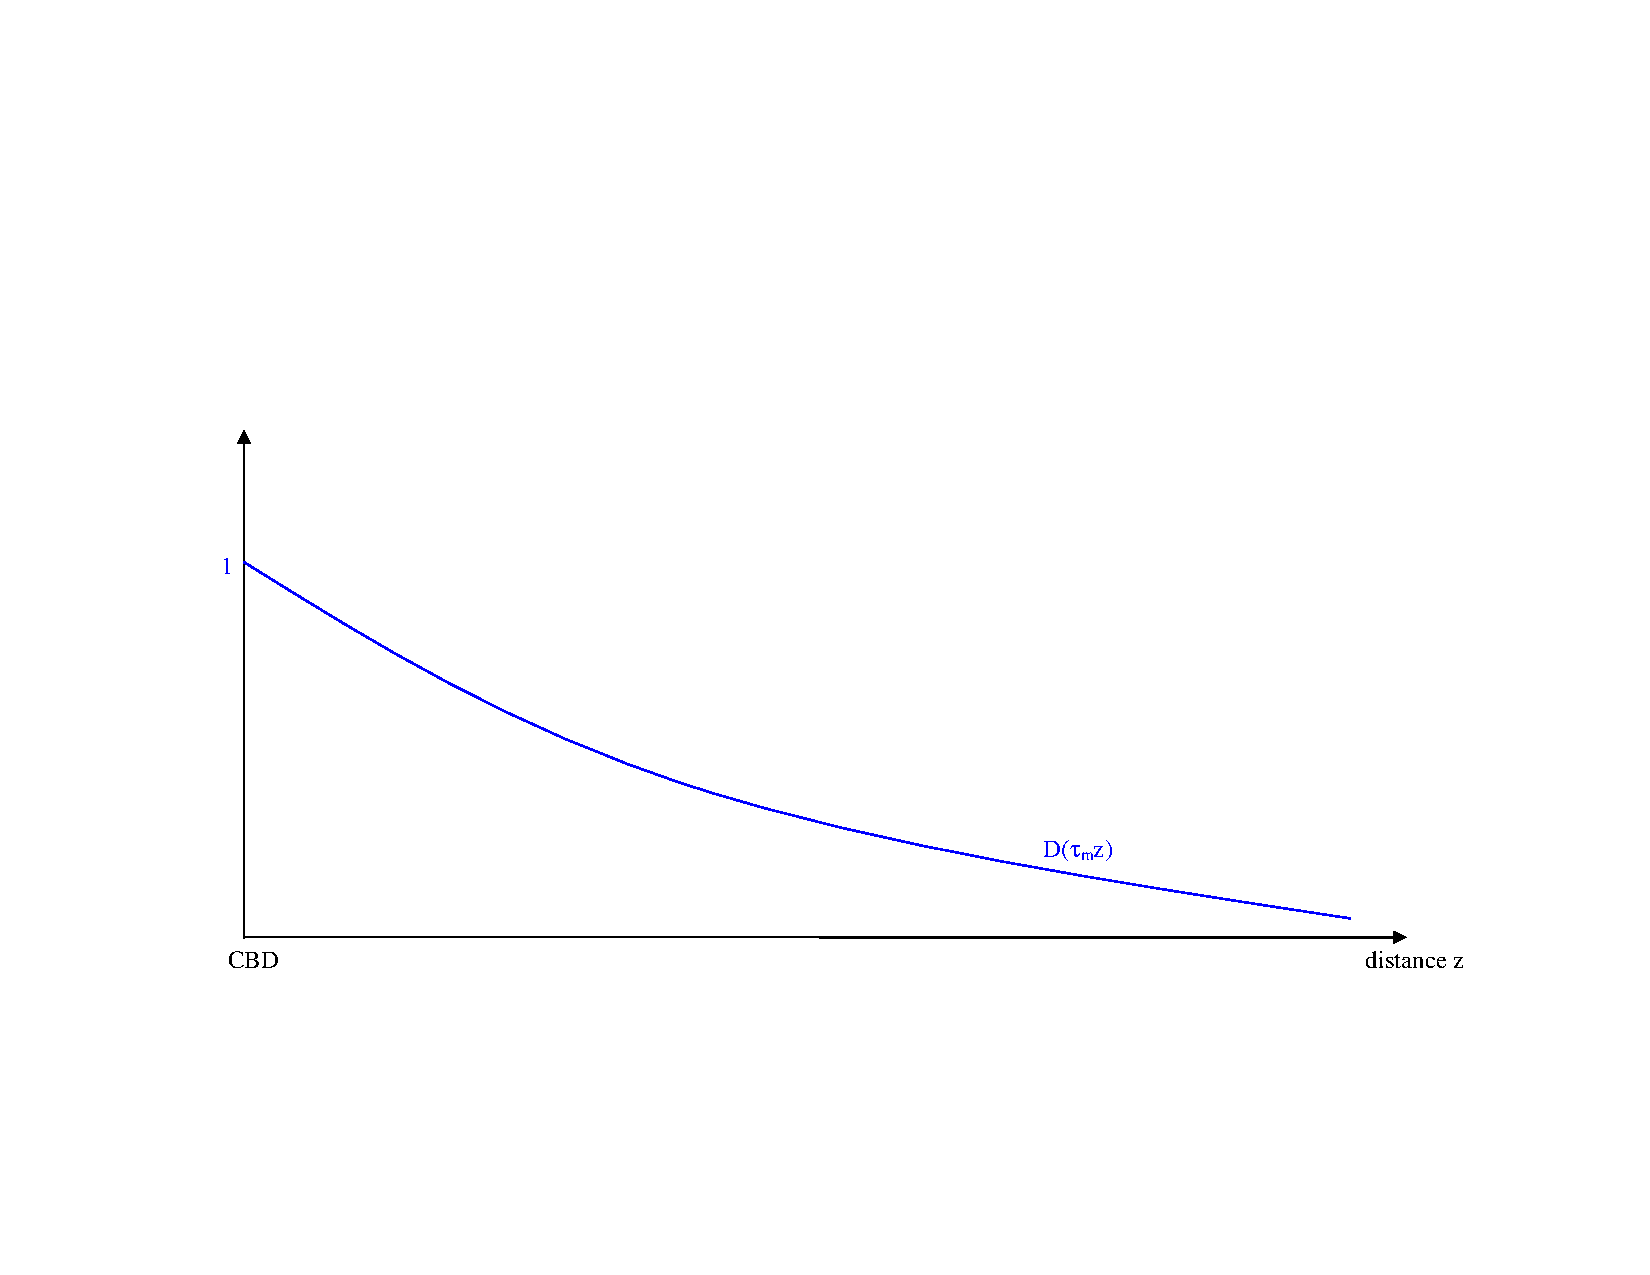
\includegraphics[width=0.7\linewidth]{figures/Dz}
  \vspace*{-1em}
  \caption{Iceberg transport costs and distance}\label{fig:Dz}
\end{figure}

The profit of a firm in industry $i$ $z$ miles from the center is
\[
\pi_i(z,l,n) = p_iD(\tau_i z)A_il_i(z)^\beta n_i(z)^{1-\beta} - wn_i(z) - r(z)l_i(z),
\]
where $w$ is the wage rate, and $r(z)$ is the land rent in location $z$.\footnote{Note that the wage does not depend on the location. We assume that all employees are hired in the CBD.}

To maintain the convenient iceberg nature of transport costs for residential location, we assume that commuting $z$ miles costs a $1-D(\tau_h z)$ fraction of the consumption bundle (including manufacturing, services and housing). One can think of this as time lost in commuting from enjoying the consumption goods. Then the budget constraint of a household at location $z$ is
\[
p_m m(z) + p_s s(z) + p_h(z) h(z) \le (w+T)D(\tau_h z).
\]
Expenditure on the manufactured good, on services and housing has to be less than the total income of the household net of commuting costs. Total income is made of wages $w$ and rental income $T$. Importantly, neither source of income depends on the choice of residential location. Rental income is derived from the plot of land the household \emph{owns}, not from where it \emph{resides}. Perfect rental markets ensure that the ownership of the land is irrelevant for location decisions.


\subsection{Equilibrium}
\begin{definition}
 An \emph{equilibrium} in this economy is a collection of land and labor allocations and goods prodiction in each industry $i$ at each location $z$, *** such that
\begin{enumerate}
 \item firms maximize profits (and hence choose their location optimally),
 \item households maximize utility (and hence choose their residence optimally),
 \item manufacturing and service markets clear at the CBD,
 \item the labor market clears at the CBD,
 \item land markets clear at each location.
\end{enumerate}

\end{definition}

We first characterize the profit maximization problem. The first-order condition for profit maximum is
\[
p_i D(\tau_i z)A_i \le r(z),
\]
with equality when there is positive production. This pins down industry $i$'s bid rent function,
\[
R_i(z,p_i) = p_i D(\tau_i z)A_i.
\]
This is the maximum rent the industry is willing to pay at location $z$. It is decreasing in $z$. Note that, all else equal, the bid rent function is steeper for services because $\tau_s>\tau_m$. Figure ***





Consumer's choice can be broken down to two steps. The first step is the allocation of consumption expenditure at a given location to manufacturing, services, and housing. Once that decision is made optimally, the resulting utility at location $z$ will be characterized by the indirect utility function of income and prices.

Suppose the level of utility is $u$ in all locations (this is equalized across locations, but the level $u$ is endogenous).

To achieve utility $u$ at location $z$,
    \[
    u = \frac{D(\tau_h z) I}{P[\Phi(p_m,p_s),r(z)/A_h]}.
    \]
    \item Bid rent function
    \[
    R_h(z) = A_h\Phi(p_m,p_s)P_2^{-1}\left[\frac{D(\tau_h z) I}{u\Phi(p_m,p_s)}\right].
    \]
	\item For example, with Cobb--Douglas utility,
\[
R_h(z) = A_h\left[\frac{D(\tau_h z) I}{up_m^{\alpha}p_s^{\beta}}\right]^{1/\gamma}.
\]


Then the bid rent function of households is such that
\[
P(p_m,p_s,R_z) = \frac Iu  D(\tau_h z).
\]

For given income and good prices, the optimal location choice of households determines their bid rent function, $R_h(z,I,p_m,p_s)$. Because the indirect utility function is homogeneous of degree zero in $I$, $p_m$, $p_s$ and $r(z)$, the bid rent function is homogeneous of degree one in $I$, $p_m$ and $p_s$.

\begin{proposition}
An equilibrium exists, is unique, and exhibits the following spatial structure. Residents live closest to the center, followed by service establishments, and then by manufacturing establishment.
\end{proposition}

(It probably suffices to set $\tau_h>\tau_s>\tau_m$.) Let $z_1$ denote the boundary of the service sector, and $z_2>z_1$ the boundary of the manufacturing sector. The city boundary is denoted by $z_3 = 1/\tau_m$. It is not feasible to transport manufactured goods from outside this boundary.

\subsection{Productivity growth}
We conduct the following comparative statics. We increase $A_m$ and $A_s$ proportionally (so that productivity growth is neutral), and ask what happens to industry location ($z_1$, $z_2$) and relative prices.
\begin{proposition}[Balassa--Samuelson and the sprawl]
 Assume that $A_m/A_s$ is constant. The the relative price of services increases with development if and only if residential land increases with development.
\end{proposition}

\begin{proposition}[Balanced growth]
Productivity growth does not change the relative price of services if either
      (i) housing productivity grows at the same rate,
      or (ii) demand for housing is Cobb--Douglas.
\end{proposition}

\subsection{A special case}
To explore the properties of the model further, we make the following additional assumptions.
There is no technical progress in housing, $A_h$ is constant. Utility is Cobb--Douglas in goods, Leontief in housing,
\[
u(m,s,h) = \min\{m^\gamma s^{1-\gamma} ,h/H\}.
\]
Transport costs are exponential,\footnote{This corresponds to a constant hazard rate. If, for example, during each mile transported there is a 1\% chance that the goods gets stolen, the iceberg shipping cost is $\exp(-0.01 z)$.}
\[
D(\tau z) = \exp(-\tau z).
\]
These assumptions lead to a closed-form solution. ***

The strength of the Balassa--Samuelson effect can be obtained by (log-)differentiating the relative price of services with respect to productivity:
\[
\frac{d\ln (p_s/p_m)}{d\ln A} = \frac{(\tau_s-\tau_m)z_1}{1+\Bar\tau z_1/\beta}
\]
The Balassa--Samuelson effect is stronger if (i) trade cost differential between the two industries is large,       (ii) land occupied by residential housing is large, and (iii) the land share in production is large.



As productivity increases,
\begin{enumerate}
    \item residential land increases,
    \item home prices increase,
    \item the rent gradient becomes steeper,
	\item tradable industries move away from center,
    \item services become more expensive,
	\item labor productivity increases faster in manufacturing.
%	\item employment becomes more concentrated.
\end{enumerate}
\begin{enumerate}
	\item[7.] All of these effects are stronger for more densely populated countries.
\end{enumerate}



%% keep tau so that we can do comparative statics


\section{Empirical results}\label{empirics}
In this section, we present some suggestive evidence supporting the
main mechanisms of the model.

\subsection{Urbanization and prices}
Figure \ref{fig:penn_joint} shows the well known result that higher
per capita income is related to higher aggregate price level. We also show that
higher urbanization increases this influence of per capita income on
the price level and has a similar effect of the relative
non-tradable/tradable prices in standard cross-country regressions.

\begin{figure}[h!]
\centering
  % Requires \usepackage{graphicx}
  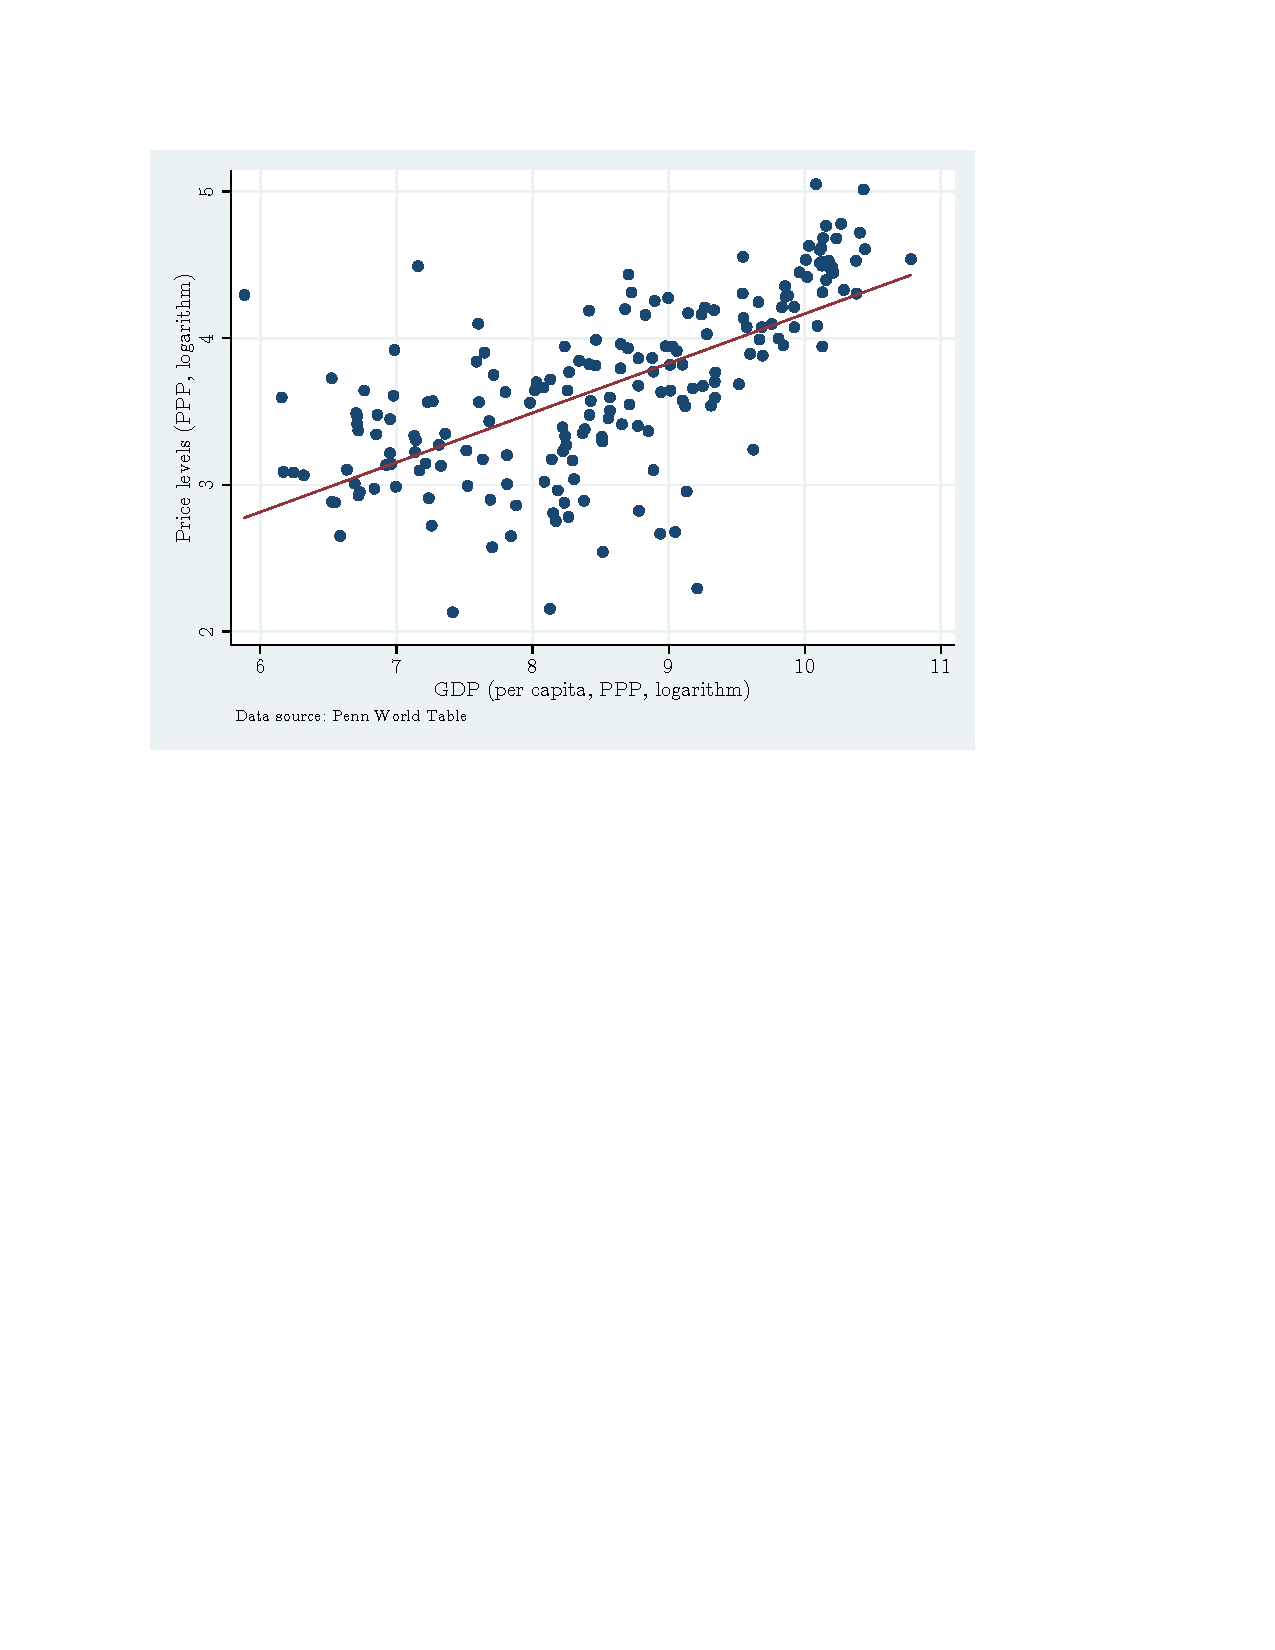
\includegraphics[width=0.7\linewidth]{figures/sc_penn_joint}\\
  \caption{Price levels and per capita GDP across countries}\label{fig:penn_joint}
\end{figure}

Two related, but distinct measures we can use to compare the
urbanization level of a country are the proportion of urban
population and the population density, both available for a large
number of countries from the World Development Indicators database.
As our main question is the difference in the 'closeness of
residents', both measures are imperfect,\footnote{Population
weighted population-density would be a measure which would express
the best the scarcity of land in a country. We are about to develop
this measure using the detailed population and land area measures of
the LandScan database.} but we consider the proportion of urban
population a better measure, as it can be expected to capture the
clustering of the population better than just the average population
density in a country. As the the definition of urban population is
different in every country, however, the cross-country results
should be treated with some caution.

Using the proportion of urban population to divide the sample
equally to more rural and more urbanized countries, Figure
\ref{fig:pennX} shows the cross-country relationships of the (log) price levels
and the (log) per capita GDP for both groups, using data from the
Penn World Table. The graphs shows, in line with our conjecture,
that the relationship between income and the price level is stronger
among more urbanized countries. It also shows that the comparison is
valid as there are reasonable variation in per capita GDP for both
groups, even if there are clearly more high-income countries among
the more urbanized ones.

\begin{figure}[h!]
\centering
  % Requires \usepackage{graphicx}
  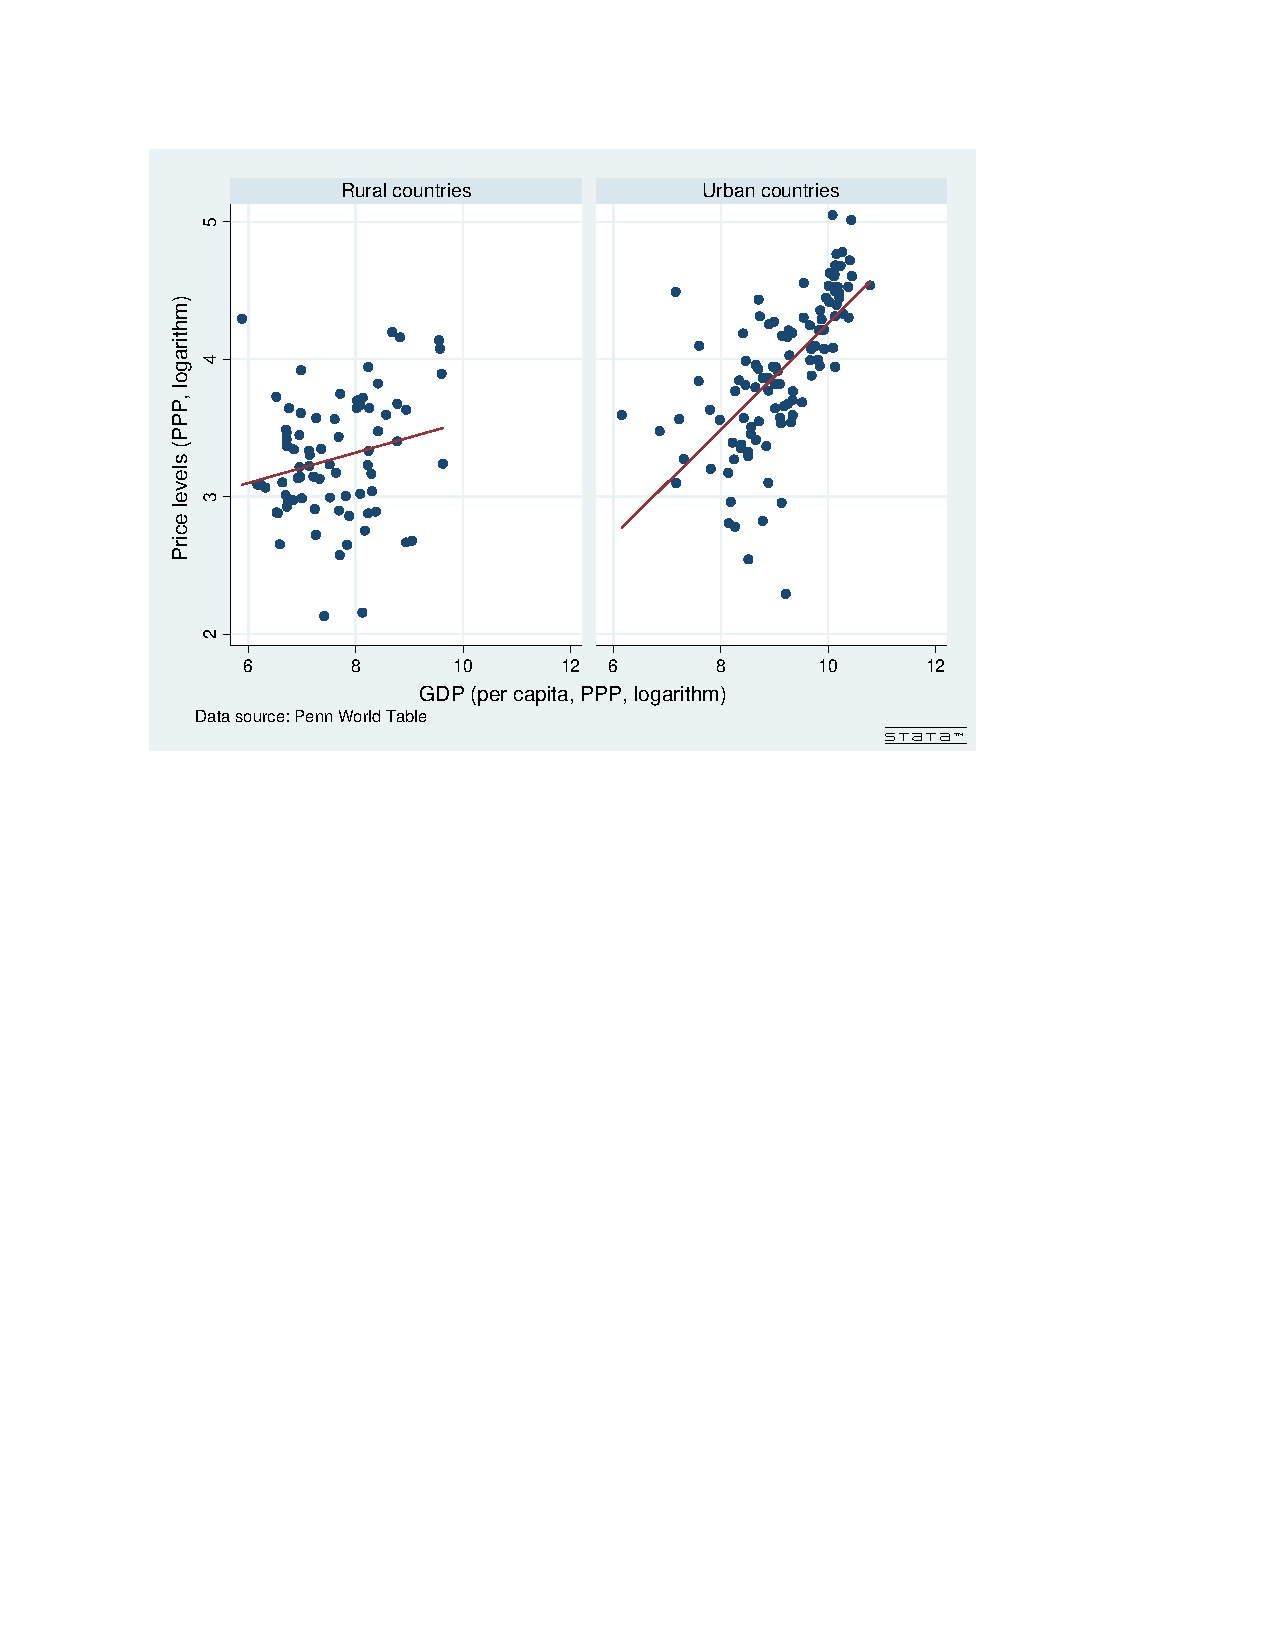
\includegraphics[width=0.7\linewidth]{figures/sc_penn}\\
  \caption{Development, urbanization, and price levels}\label{fig:pennX}
\end{figure}


To approach the question more formally, we estimated some
regressions in the following form
\begin{equation}
\log{P}=\alpha_1+\alpha_2\log Y+\alpha_3Z+\alpha_4(Z-\bar{Z})(\log Y-\overline{\log Y})+\varepsilon,
\end{equation}
where $P$ refers to the various price measures, Y is the measure of
GDP, and $Z$-s are the different urbanization measures. Our main
interest is in the (demeaned) cross-term, as it can be expected to
capture how the level of urbanization influences the relationship
between the output and the price measures.

Our main price measure is the comparable price level available for
over 180 countries from the Penn World Table.\footnote{The sample
extends the 115 benchmark countries, that directly participated the
1996 round of the International Comparison Project(ICP), by using
somewhat less reliable price data and other observable variables.
Our results are robust to restricting the sample to the benchmark
countries.} To check the robustness of the results, we also
calculated a non-tradable/tradable relative price index
($P_{NT}/P_{T}$) using the basic heading level price data for
consumption for the 1996 benchmark ICP countries. This relative
price is more in line with the Balassa-Samuelson proposition
implying that the main reason of the price level difference is the
relatively more expensive non-tradable prices. The measure, however,
can be expected to be less reliable than the aggregate price level
as the non-tradable prices, like services, tend to be less
comparable internationally than tradable prices,

\begin{table}[h!]
\caption{Balassa-Samuelson regressions with urbanization (Robust
standard errors are in parentheses)} \center \label{tab:BS}
\begin{tabular}{c|cc|cc}
  \hline\hline
  Explanatory & \multicolumn{4}{c}{Dependent variables} \\
  variables &\multicolumn{2}{c}{$\log P$} & \multicolumn{2}{c}{$\log(P_{NT}/P_T)$} \\ \hline
  $\log Y$ & \textbf{0.25} & \textbf{0.34} & \textbf{0.28}   & \textbf{0.33} \\
           & (0.05)        & (0.03)        & (0.07)          & (0.05)        \\
  urban    & \textbf{0.61} &               & 0.12            &               \\
           & (0.21)        &               & (0.34)          &               \\
  urbanX   & \textbf{0.38} &               & \textbf{0.43}   &              \\
           & (0.11)        &               & (0.19)          &              \\
  log(density) &           & -0.02         &                 & -0.02        \\
             &             & (0.02)        &                 &  0.04        \\
  densityX &               & \textbf{0.05} &                  & 0.01         \\
           &               & (0.02)        &                 & 0.02         \\
  constant & \textbf{1.13} & \textbf{0.82} & \textbf{-2.96}  & \textbf{-3.13}\\
           & (0.31)        & (0.26)        & 0.50            & (0.41)        \\ \hline
  No. of obs. & 186        & 183           & 113             & 113          \\
  $R^2$    & 0.50          & 0.46          & 0.38            & 0.34  \\
  \hline\hline
\end{tabular}
\end{table}

Table \ref{tab:BS} implies that the regressions mostly support our
conjectures. The first two columns use the (log) price levels as
dependent variables, while the last two uses the (log) relative
non-tradable/tradable prices. For both dependent variables, we
present two regressions with the two urbanization measures. 'Urban'
is the proportion of urban population, and 'density' is the
population density; and 'urbanX' and 'densityX' are the demeaned
output-urbanization cross terms.

In line with well known previous results, higher per capita output
increases both the price level and the relative prices across
countries, but this relationship is significantly influenced by the
level of urbanization, even after controlling for direct price
effects of the urbanization. Looking at the first regression, we
have found that 1 percent higher per capita output increases the price
level by 0.25 percent for average level of urbanization (54 percent), and 1 percent
higher urbanization has a further 0.61 percent direct effect. The cross
effect, however, implies that the effect of output on the prices
would be close to 0 under the (extreme) case of 0 urbanization
($0.25-0.54\cdot0.38=0.05$) and would be over 0.4 in case of full
urbanization. The effects using the relative prices are similar
supporting the conjecture that the price differences are the result
of different non-tradable prices. Using the population density as
explanatory variable still supports the effect using the price
level, though it turns out to be insignificant for our sample in
explaining the cross country relative price differences.

\subsection{Industry location}
An important starting point of the model is the assumption that
non-tradables have to be produced close to the consumers. An
implication of this spatial assumption is that higher urbanization
of the population in an area would imply higher relative employment
in the non-tradable sectors than in the tradeable ones. We have
examined this mechanism by looking at the US Census 2000
data.\footnote{The more detailed survey covering approximately 15 percent
of the households contains detailed (NAICS 2 digit level)
information about the industry level employment, while the general
short survey contains information about the urban population and
population density according to various geographic areas}

Figure \ref{fig:nt-states} shows the relationship between the proportion of urban
population and the relative non-tradable/tradable employment for US
states, strongly supporting the conjectured positive relationship.

\begin{figure}[h!]
\centering
  % Requires \usepackage{graphicx}
  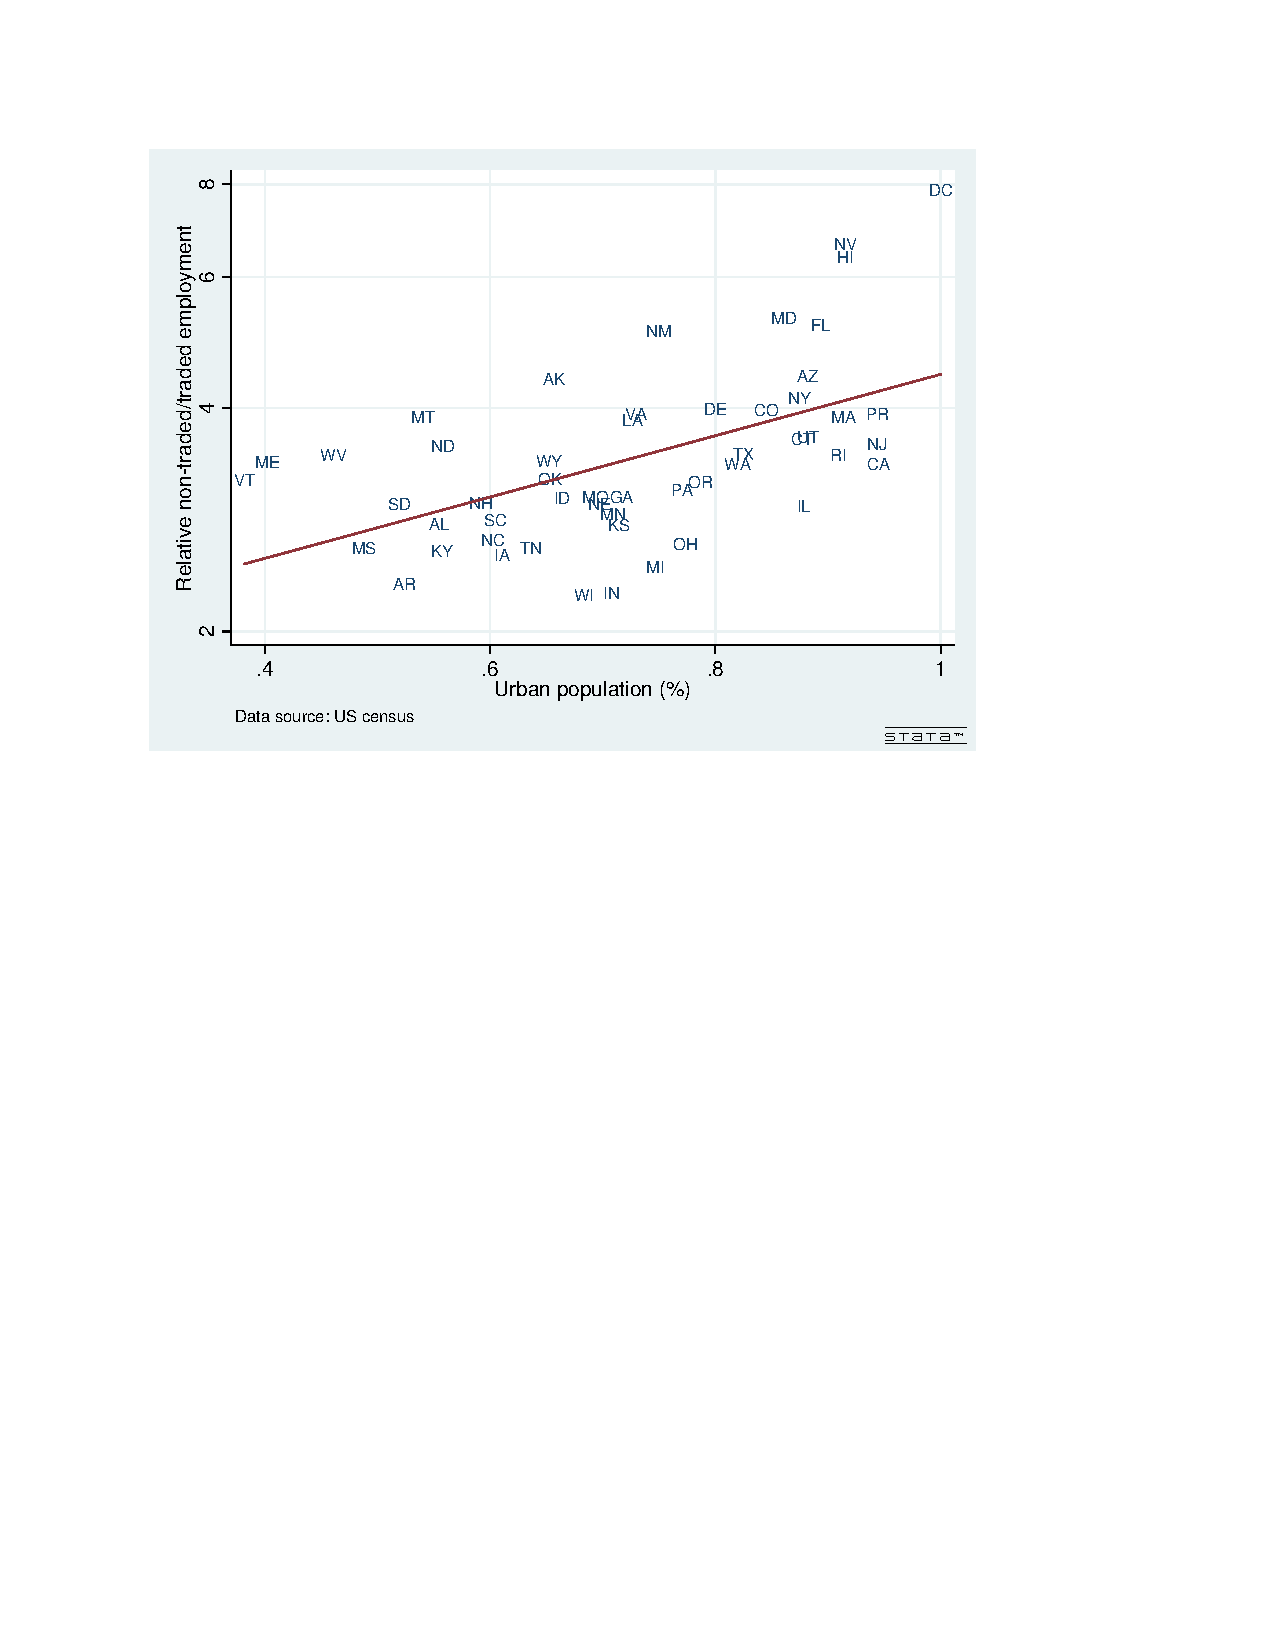
\includegraphics[width=0.7\linewidth]{figures/sc_state}\\
  \caption{Urbanization and non-traded employment in U.S.~states}\label{fig:nt-states}
\end{figure}


To examine the effects more formally, we used US county level data.
The advantage of using counties is that it can capture the
population clustering better than state level data and covers the
whole country, though a potential problem is that if a large number
of the employees live and work in different
counties.\footnote{Metropolitan statistical areas are a possible
alternatives taking commuting habits into consideration, but,
naturally, do not covering the whole country. Our regressions are
robust to using these areas as well.} As before, we used the
proportion of urban population and population density as measures of
urbanization and also included the (log) per capita median income
within the county.

\begin{table}[h!]
\center \caption{Urbanization and relative NT/T employment (Robust
standard errors are in parentheses)}
\begin{tabular}{c|cc}
  \hline\hline
  Explanatory & \multicolumn{2}{c}{Dependent variable} \\
  variables & \multicolumn{2}{c}{$\log (N_{NT}/N_T)$} \\ \hline
  urban         & \textbf{0.62} &  \\
                & (0.02)        &  \\
  log(density)  &               & \textbf{0.07} \\
                &               & (0.01) \\
  log(income)   & \textbf{0.11} & \textbf{0.18} \\
                & (0.02)        & (0.03) \\
  constant      & -0.53         & \textbf{-1.18} \\
                & (0.28)        & (0.30) \\ \hline
  $R^2$         & 0.20          & 0.10 \\
  No. of obs.   & 3218          & 3218 \\ \hline\hline
\end{tabular}
\end{table}

The results show that even after correcting for the median income,
the level of urbanization -- measured in the proportion of urban
population or population density -- significantly increases the
proportion of employees working in non-tradable sectors supporting
our spatial correlation assumption.

\subsection{Land prices and income}
The effects of development on the price of land is a major mechanism
in our model influencing the relative price of services. To have a
first look at the question, we use the dataset constructed by Davis and
Palumbo (2008) who created implied residential land value data for 46
large U.S.~metropolitan areas. To get this data, the authors use
regional data on construction costs and decompose the value of an
average home to replacement value and land value.

\begin{figure}[h!]
\centering
  % Requires \usepackage{graphicx}
  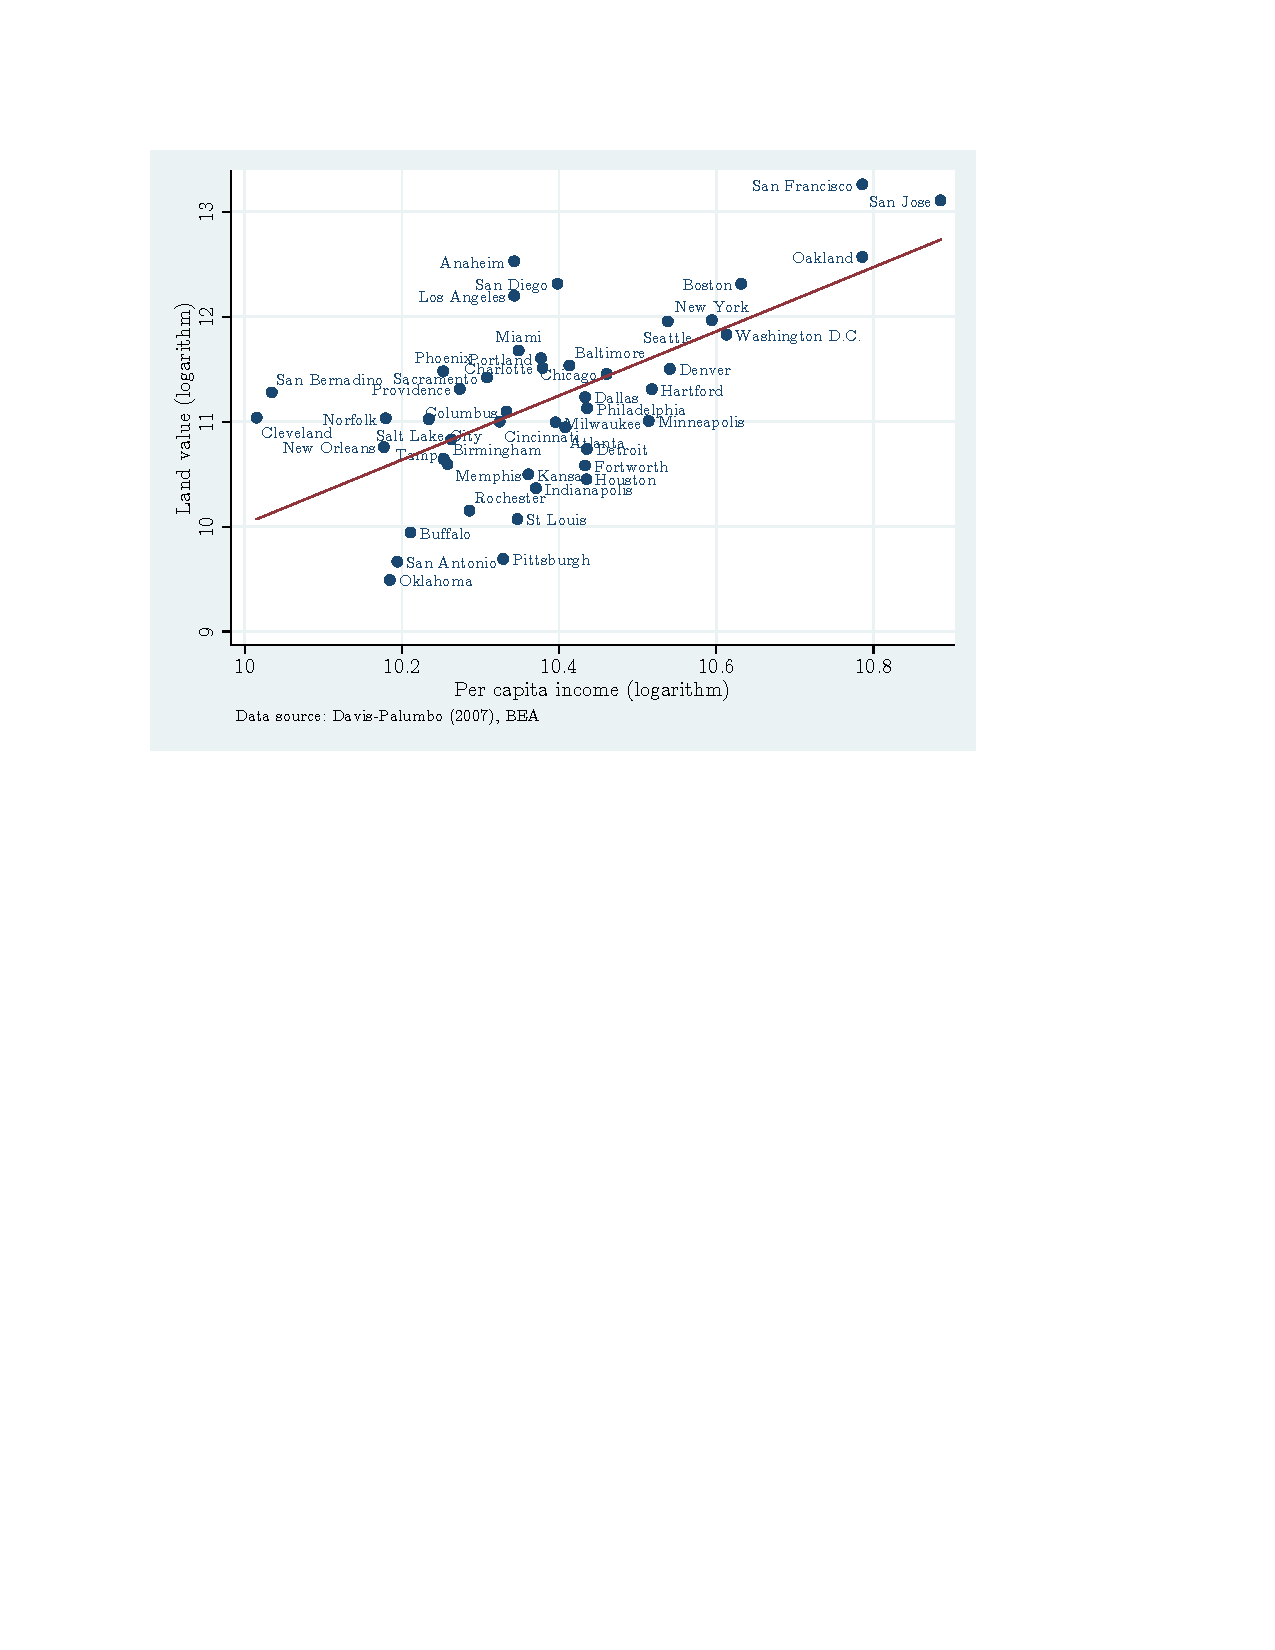
\includegraphics[width=0.7\linewidth]{figures/sc_davis}\\
  \caption{Land prices and income across large US cities}\label{fig:land}
\end{figure}

Figure \ref{fig:land} shows the (log) price of land as a function of
per capita income for the U.S.~cities. It strongly supports our
conjecture that higher income areas face more appreciated land
prices.

Table \ref{tab:land} shows the estimated effects of income on the
land prices, the replacement values (constr) and home values
controlling for the size of the metropolitan areas. The regressions
show that the regional income influences all the values, but it has
the largest effect on the land prices with an amplification factor
of 2.8. This is consistent with our model, in which the complementarity between land and consumption leads to an amplified response of rents to income.

\begin{table}[h!]
\center \caption{Land prices and income (Robust standard errors are
in parentheses)} \label{tab:land}
\begin{tabular}{c|ccc}
  \hline\hline
  Explanatory & \multicolumn{3}{c}{Dependent variable} \\
  variables & log(land) & log(constr) & log(home) \\ \hline
  log(income)    & \textbf{2.77}   & \textbf{0.38}  & \textbf{1.66}\\
                 & (0.67)          & (0.11)         &  (0.38)\\
  log(population)& 0.13            &  0.02          &  0.05\\
                 & (0.18)          & (0.03)         &  0.10\\
  constant       & \textbf{-19.47} & \textbf{7.38}  &  -5.83\\
                 & (6.35)          & (1.12)         &  (3.53)\\ \hline
  $R^2$          & 0.42            & 0.25           &   0.52\\
  No. of obs.    & 46              & 46             &   46   \\ \hline\hline
\end{tabular}
\end{table}

\section{Conclusion}
[TO BE WRITTEN]

\begin{thebibliography}{99}
\bibitem{Balassa64} Balassa, B., 1964, ``The Purchasing-Power Parity Doctrine: A
Reappraisal,'' \emph{Journal of Political Economy}, 584-596.
\bibitem{Davis07} Davis, M. A. and Heathcote, J., 2007, ``The Price and Quantity of Residential Land in the United States,'' \emph{Journal of Monetary Economics} 54:2595-2620.
\bibitem{Davis07} Davis, M. A. and Palumbo, M. G., 2008, ``The Price
of Residential Land in Large U.S. Cities,'' \emph{Journal of Urban Economics}, 63:352--384.
\bibitem{} Davis, M. A. and Ortalo-Magne, F., 2007, ``Household Expenditures, Wages, Rents,'' working paper.
\bibitem{Heston06} Heston, A., R. Summers and B. Aten, 2006, Penn World Table Version 6.2, \emph{Center for International Comparisons of Production, Income and Prices at the University of
Pennsylvania}
\bibitem{Klenow07} Hsieh, C.T and Klenow, P.J, ``Relative Prices and
Relative Prosperity,'' \emph{The American Economic Review}, 562-585.
    \bibitem{Obstfeld99} Obstfeld, M. and Rogoff, K., 1996, \emph{Foundations of International
Macroeconomics}, The MIT Press, Cambridge MA
    \bibitem{Samuelson64} Samuelson, P. A. , 1964, ``Theoretical Notes on Trade
Problems,'' \emph{The Review of Economics and Statistics}, 145-154.
    \bibitem{} Tang, X., 2007, ``The Rich Neighborhood Effect versus the Balassa-Samuelson Effect: An Income-Based Explanation of International Price Level Differences,'' working paper.
\end{thebibliography}

\end{document}
